\RequirePackage{currfile} 
\documentclass{beamer}
%%%%%%%%%%%%%%%%%%%%%%%%%%%%%%%%%%%%%%%%%
% Beamer Presentation
% LaTeX Template
% Version 1.0 (10/11/12)
%
% This template has been downloaded from:
% http://www.LaTeXTemplates.com
%
% License:
% CC BY-NC-SA 3.0 (http://creativecommons.org/licenses/by-nc-sa/3.0/)
%
%%%%%%%%%%%%%%%%%%%%%%%%%%%%%%%%%%%%%%%%%

%----------------------------------------------------------------------------------------
%	PACKAGES AND THEMES
%----------------------------------------------------------------------------------------




\mode<presentation> {

% The Beamer class comes with a number of default slide themes
% which change the colours and layouts of slides. Below is a list
% of all the themes, uncomment each, in turn, to see what they look like.

%\usetheme{default}
%\usetheme{AnnArbor} %yellow
\usetheme{Antibes}
%\usetheme{Bergen}
%\usetheme{Berkeley}
%\usetheme{Berlin}
%\usetheme{Boadilla}
%\usetheme{CambridgeUS}
%\usetheme{Copenhagen}
%\usetheme{Darmstadt}
%\usetheme{Dresden}
%\usetheme{Frankfurt}
%\usetheme{Goettingen}
%\usetheme{Hannover}
%\usetheme{Ilmenau}
%\usetheme{JuanLesPins}
%\usetheme{Luebeck}
%\usetheme{Madrid}		
%\usetheme{Malmoe}
%\usetheme{Marburg}
%\usetheme{Montpellier}
%\usetheme{PaloAlto}
%\usetheme{Pittsburgh}
%\usetheme{Rochester}
%\usetheme{Singapore}
%\usetheme{Szeged}
%\usetheme{Warsaw}

% As well as themes, the Beamer class has a number of colour themes
% for any slide theme. Uncomment each of these, in turn, to see how it
% changes the colours of your current slide theme.

%\usecolortheme{albatross}


\usecolortheme{beaver}
%\usecolortheme{beetle}
%\usecolortheme{crane}
%\usecolortheme{dolphin}
%\usecolortheme{dove}
%\usecolortheme{fly}
%\usecolortheme{lily}
%\usecolortheme{orchid}
%\usecolortheme{rose}
%\usecolortheme{seagull}
%\usecolortheme{seahorse}
%\usecolortheme{whale}
%\usecolortheme{wolverine}

\setbeamertemplate{footline} % To remove the footer line in all slides uncomment this line
%\setbeamertemplate{footline}[frame number] % To replace the footer line in all slides with a simple slide count uncomment this line

%\setbeamertemplate{navigation symbols}{} % To remove the navigation symbols from the bottom of all slides uncomment this line

\setbeamercovered{transparent} % Fait apparaître les animations en grisé (utile pour la conception, mais peut être commenté lors de la remise du document final)

% Pour utiliser une police à empattements partout
\usefonttheme{serif}

% Pour rajouter la numérotation des frames dans les pieds de page
\newcommand*\oldmacro{}%
\let\oldmacro\insertshorttitle%
\renewcommand*\insertshorttitle{%
  \oldmacro\hfill%
  \insertframenumber\,/\,\inserttotalframenumber}

}

\usepackage{graphicx} % Allows including images
\usepackage{booktabs} % Allows the use of \toprule, \midrule and \bottomrule in tables



% Les autres packages utiles  notamment pour le français, les accents ou Python
\usepackage{natbib}         % Pour la bibliographie
\usepackage{url}            % Pour citer les adresses web
\usepackage[T1]{fontenc}    % Encodage des accents
\usepackage[utf8]{inputenc} % Lui aussi

\usepackage{numprint}       % Histoire que les chiffres soient bien
\usepackage{subfig}
\usepackage{amsmath}        % La base pour les maths
\usepackage{mathrsfs}       % Quelques symboles supplémentaires
\usepackage{amssymb}        % encore des symboles.
\usepackage{amsfonts}       % Des fontes, eg pour \mathbb.

\usepackage{cancel}


%\usepackage[svgnames]{xcolor} % De la couleur

%%% Si jamais vous voulez changer de police: décommentez les trois 
%\usepackage{tgpagella}
%\usepackage{tgadventor}
%\usepackage{inconsolata}

%%% Pour L'utilisation de Python
\usepackage{minted}
\usemintedstyle{friendly}

\usepackage{graphicx} % inclusion des graphiques
\usepackage{wrapfig}  % Dessins dans le texte.

\usepackage{tikz}     % Un package pour les dessins (utilisé pour l'environnement {code})
\usepackage[framemethod=TikZ]{mdframed}
\usetikzlibrary{snakes}


% Les macros et raccourcis personnels
%% Ce fichier contient toutes les macros que vous pouvez avoir envie de définir 
% si vous les utilisez plusieurs fois dans le document.

\PassOptionsToPackage{svgnames}{color}

% Un environnement pour bien présenter le code informatique
\newenvironment{code}{%
\begin{mdframed}[linecolor=green,innerrightmargin=30pt,innerleftmargin=30pt,
backgroundcolor=black!5,
skipabove=10pt,skipbelow=10pt,roundcorner=5pt,
splitbottomskip=6pt,splittopskip=12pt]
}{%
\end{mdframed}
}

% Des parenthèses, crochets et accolades qui s'adaptent automatiquement à la 
% taille de ce qu'il y a dedans
\newcommand{\pa}[1]{\left(#1\right)}
\newcommand{\pac}[1]{\left[#1\right]}
\newcommand{\paa}[1]{\left\{#1\right\}}


% On définit le titre et l'auteur du document

% L'argument optionnel (entre crochets) donne le titre qui sera mis sur chaque slide
\title[]{  PLS: Exploiting the Physical Medium for Securing Resource-Constrained Networks}
\author{Chrysanthi Paschou} % Votre nom
% L'épreuve (car on n'a pas le droit de signaler sa provenance à un concours) (là encore, l'argument optionnel apparaît sur chaque slide)

\institute[TIPE]{\textcolor{red}{\textbf{University of Bristol}}}
%\date{\today} 

% On démarre le document proprement dit
\begin{document}

% Rien d'autre à faire qu'afficher le titre

\begin{frame}
\titlepage 
\vspace*{-1cm}
\begin{center}

\includegraphics[width=0.13\linewidth]{preambule/logos/bristolcrest_colour.pdf}
\end{center}
\vspace{-0.32cm}
{\small
Supervisory Team: Prof A. Doufexi \& Prof O. Johnson\\
Mentorship: Toshiba Research \& Innovation Laboratory, Bristol}
\end{frame}


% La table des matières utilise ce que vous donnez aux commandes \section et 
% \subsection tout au long de la présentation.
\begin{frame}
\frametitle{Contexts} 
\tableofcontents 
\end{frame}


% Titre de la premiere partie
\section{Introduction}
\subsection{Motivation}
%%%%%%%%%%%%%%%%%%%%%%%%%%%%%%%%%%%%%%%%%%%%%%%%
% Première diapo
%%%%%%%%%%%%%%%%%%%%%%%%%%%%%%%%%%%%%%%%%%%%%%%%
\begin{frame}{Limitations of Traditional Ways of Security}
\begin{itemize}
    \item<1-> Rapid 5G adoption increased connected devices, often with memory and energy constraints;
    \item<2-> Traditional security methods (e.g., public key cryptography) are impractical due to resource-intensive calculations;
    \item<3-> Inadequate security mechanisms in low-power/low-memory devices lead to fixed or low entropy keys, posing network vulnerabilities;
    \item<4-> PKC-based authentication fails to protect against person-in-the-middle attacks in short-range communications systems.
\end{itemize}


%\begin{itemize}
 %   \item<1-> The rapid adoption of 5G technology has led to a significant increase in the number of connected devices, many of which have constraints on memory and energy.
    
  %  \item<2-> Traditional security methods, such as public key cryptography (PKC), involve intensive calculations and require excessive resources for low-cost devices, making them impractical.
   % \item<3-> Inadequate security mechanisms for low-power/low-memory devices can result in fixed or low entropy keys, posing vulnerabilities to the entire network.
    %\item<4-> PKC-based authentication does not protect against person-in-the-middle attacks, which are prevalent in short-range communications systems like keyless entry and contactless payments.
 %\end{itemize}   
\end{frame}

\begin{frame}{PLS as a potential solution}
    Physical Layer Security (PLS) encompasses
    \begin{itemize}
        \item keyless PLS;
        \item key-based PLS;
        \item the recent branch of Physical Layer Authentication (PLA).
        \end{itemize}
    \begin{center}
        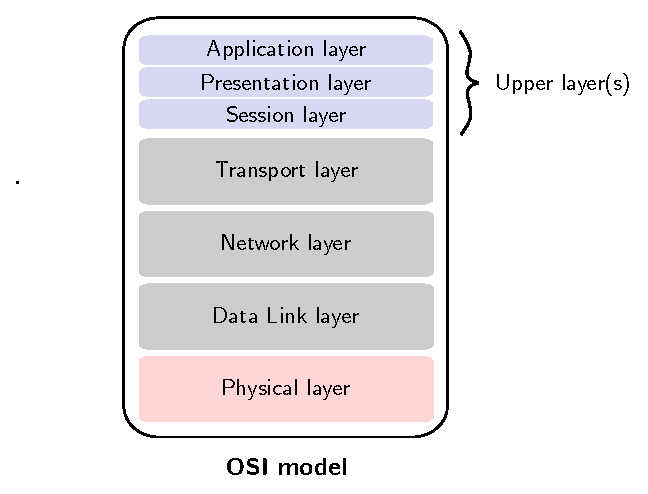
\includegraphics[width = 0.6\linewidth]{slides/figures/iso.eps}
        
    \end{center}
\end{frame}


%\begin{frame}
%\frametitle{PLS as a potential solution}

%\begin{itemize}
%\item<1-> Keyless PLS utilises the inherent randomness of the physical medium to achieve confidentiality without the need for keys or a secure key exchange.
%\item<2->Key-based PLS extracts unique randomness from the physical link to generate shared secret keys for symmetric cryptography.
%\item<3->PLA identifies devices based on hardware imperfections in transmitted signals and offers faster authentication before signal demodulation and decoding.

    
%\end{itemize}

%\end{frame}

%%%%%%%%%%%%%%%%%%%%%%%%%%%%%%%%%%%%%%%%%%%%%%%%
\subsection{Contributions}

\begin{frame}{Contributions}
\framesubtitle{...to the state-of-the-art of keyless PLS}
 \begin{itemize}
  \item<1-> Introducing a novel method, namely \textit{secret splitting}, that exploits base station cooperation for confidentiality;\\\hfill{(chapter~5)}
  \item<2-> Secrecy splitting addresses one of the most challenging requirements of keyless PLS: the need for a positive secrecy gap.\hfill{(chapter~5)}
 % \item<3-> Performing analytical analysis on the proposed scheme and deriving the optimal base station allocation.\hfill{(chapter~5)}
\item[\textcolor{blue}{$\rightarrow$}]<3-> \textcolor{blue}{1} peer-reviewed publication (GLOBECOM 2020)
 
\end{itemize}

\end{frame}

%%%%%%%%%%%%
\begin{frame}{Contributions}
\framesubtitle{...to the state-of-the-art of key-based PLS}

\begin{itemize}
    \item<1-> Revising secure distance for certain geometric environments; \hfill{(chapter~4)}
    \item<2-> Presenting a practical key agreement protocol for resource-constrained networks, successfully tested in an IoT network.\hfill{(chapter~7)}
    \item[$\rightarrow$]<3->\textcolor{blue}{2} peer-reviewed publications (VTC2022, ICC2023)
\end{itemize}

\end{frame}

\begin{frame}
\frametitle{Contributions}
\framesubtitle{...to the state of the art of physical layer authentication}
\begin{itemize}
    %\item<1-> Introducing a new concept for authenticating devices in short-range systems based on the spatial and temporal properties of the {RF} channel;\hfill{(chapter~6)}
    
    \item<1-> Proposing a scheme for secure authentication of co-located devices against distance fraud and replay attacks;
    \hfill{(chapter~6)}
    
    \item<2-> Proposing a scheme for validating the proximity of a non-powered device that communicates using backscattering modulation. \hfill{(chapter~6)}
    \item[\textcolor{blue}{$\rightarrow$}]<3-> \textcolor{blue}{2} peer-reviewed publications (VTC2021, WCNC2023) \& \textbf{1} patent (in collaboration with Toshiba).
\end{itemize}

\end{frame}

\iffalse
\begin{frame}{Publications}
    \begin{itemize}
    \item[1.] C. Paschou, O. Johnson, A. Doufexi, Z. Zhu, and W.H. Chin. ``Increasing the secrecy gap in quasi-static Rayleigh channels with secret splitting.'' In 2020 IEEE Globecom Workshops (GC Wkshps, pp. 1-7. IEEE, 2020. \hfill{[chapter~5]}

    \item[2.] C. Paschou, O. Johnson, Z. Zhu, and A. Doufexi. ``A Lightweight Protocol for Validating Proximity in UHF RFID Systems.'' In 2021 IEEE 94th Vehicular Technology Conference (VTC2021-Fall), pp. 1-7. IEEE, 2021. \hfill[chapter~6]
    
    \item[3.] C. Paschou, O. Johnson, Z. Zhu, and A. Doufexi.``Re-Defining Secure Distance for CSI-based Key Generation Protocols.'' In 2022 IEEE 95th Vehicular Technology Conference (VTC2022-Spring), pp. 1-6. IEEE, 2022.\hfill[chapter~4]
    \end{itemize}
    \end{frame}

\begin{frame}{Publications}
    \begin{itemize}
    \item[4.] C.Paschou, Z. Zhu, M. Sandell.
    ``Preventing replay/relay attacks in keyless entry systems.'' Patent 54322US, Oblon, McClelland, Maier \& Neustadt, {L.L.P.}, 2022. \hfill[chapter~6]
    
    
    \item[5.] C. Paschou, O. Johnson, Z. Zhu, and A. Doufexi. ``Physical Layer Protection Against Relay/Replay Attacks for Short-Range Systems.'' In 2023 IEEE Wireless Communications and Networking Conference (IEEE WCNC 2023), pp. 1-6. IEEE, 2023.\hfill[chapter~6]
    

    \item[6.] C. Paschou, F. Raimondo, M. Gugala, D. McEwan, J. Pope, G. Oikonomou.
    ``CRICKET: A Practical Physical Layer Key Agreement Protocol for IoT Networks.'' In 2023 IEEE International Conference of Communications (IEEE ICC 2023), pp. 1-7. IEEE, 2023.\hfill[chapter~7]
\end{itemize}
\end{frame}
 \fi
%\visible<3->{
%	\begin{figure}
%	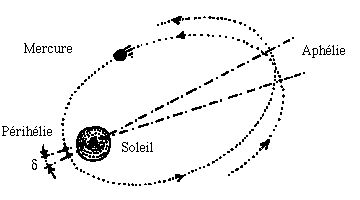
\includegraphics[width=0.8\linewidth]{figures/Fig01}
%	\end{figure}
%	}

%%%%%%%%%%%%%%%%%%%%%%%%%%%%%%%%%%%%%%%%%%%%%%%%
% Troisième diapo
%%%%%%%%%%%%%%%%%%%%%%%%%%%%%%%%%%%%%%%%%%%%%%%%
\subsection*{}
\begin{frame}{Thesis Outline}
\begin{center}
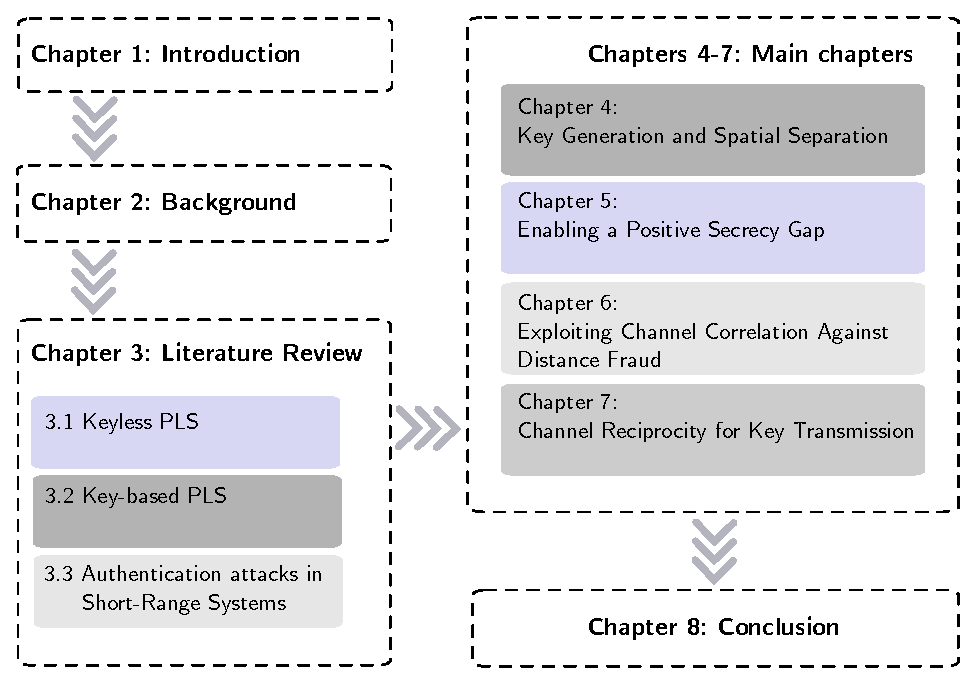
\includegraphics[width=0.9\linewidth]{slides/figures/outline.eps}
\end{center}

\end{frame}

%\input{slides/02_background}


%
\section{Literature Review}
\subsection{Survey on keyless PLS}
\begin{frame}{Wyner's wiretap channel}
\begin{figure}
    \centering
    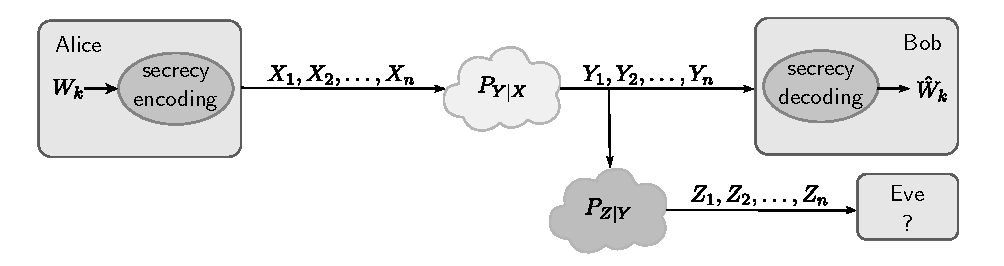
\includegraphics[scale = 0.6]{slides/figures/WiretapChannelWyner.pdf}
    \caption{The wiretap channel as introduced by Wyner in 1975. Perfect secrecy can be achieved without the use of cryptographic keys. }
    \label{fig:wyner}
\end{figure}

\onslide<2->\textbf{Limiting factor}: X-Y-Z form a Markov channel. I.e.: Eve's channel must be a degraded version of Bob's channel.
\end{frame}


\begin{frame}{The generic wiretap channel}
\begin{figure}
    \centering
    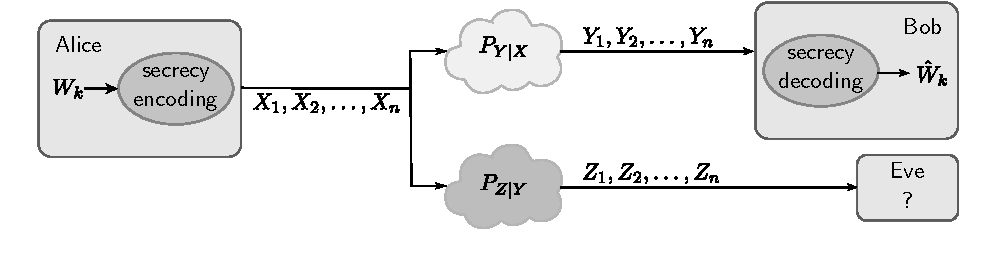
\includegraphics[scale = 0.5]{slides/figures/WiretapChannelCK.pdf}
    \caption{Csisz\'ar and K\"orner generalised Wyner's wiretap channel to include non-degraded wiretap channels.}
    \label{fig:CK}
\end{figure}


\onslide<2-> The generic model matches better the characteristics of the wireless channel.

\onslide<3->Alice transmits opportunistically at times when Bob observes a higher SNR than Eve.
\end{frame}

\begin{frame}{Common Limitations}
\begin{itemize}
    \item Knowledge of the eavesdropper's channel state information (CSI) is needed. 
    \item Secure transmission is possible only when Bob experiences a better signal quality. I.e., a positive secrecy gap is needed.
\end{itemize}

\begin{definition}
    Secrecy gap is the quality difference between the legitimate channel and the wiretap channel. 
\end{definition}

\end{frame}

\begin{frame}{Recent developments}
\begin{itemize}
\item Recent advancements in signalling processing and the employment of multiple-antenna systems  can increase the secrecy gap;

\item Secrecy coding has regained attention and started to expand beyond discrete channel models;

\item Schemes that do not require the eavesdropper’s CSI exist but they are
limited to the case of a single-antenna eavesdropper.
\end{itemize}
    
\end{frame}


\subsection{Survey on key-based PLS}

\begin{frame}{Physical Layer Key Generation}
    \begin{itemize}
        \item A new branch of PLS: key-based PLS, or, \textbf{physical layer key generation};
        \item Aims to generate symmetrical keys, thus enabling upper-layer encryption;
        \item Keys are extracted from the randomness inherited in the wireless multipath channel; 
        \item Early-test bed experimentations prove that physical layer key generation has practical value in today's systems.  
    \end{itemize}
\end{frame}

\begin{frame}{The four stages of physical layer key generation}
    
\begin{figure}
    \centering
    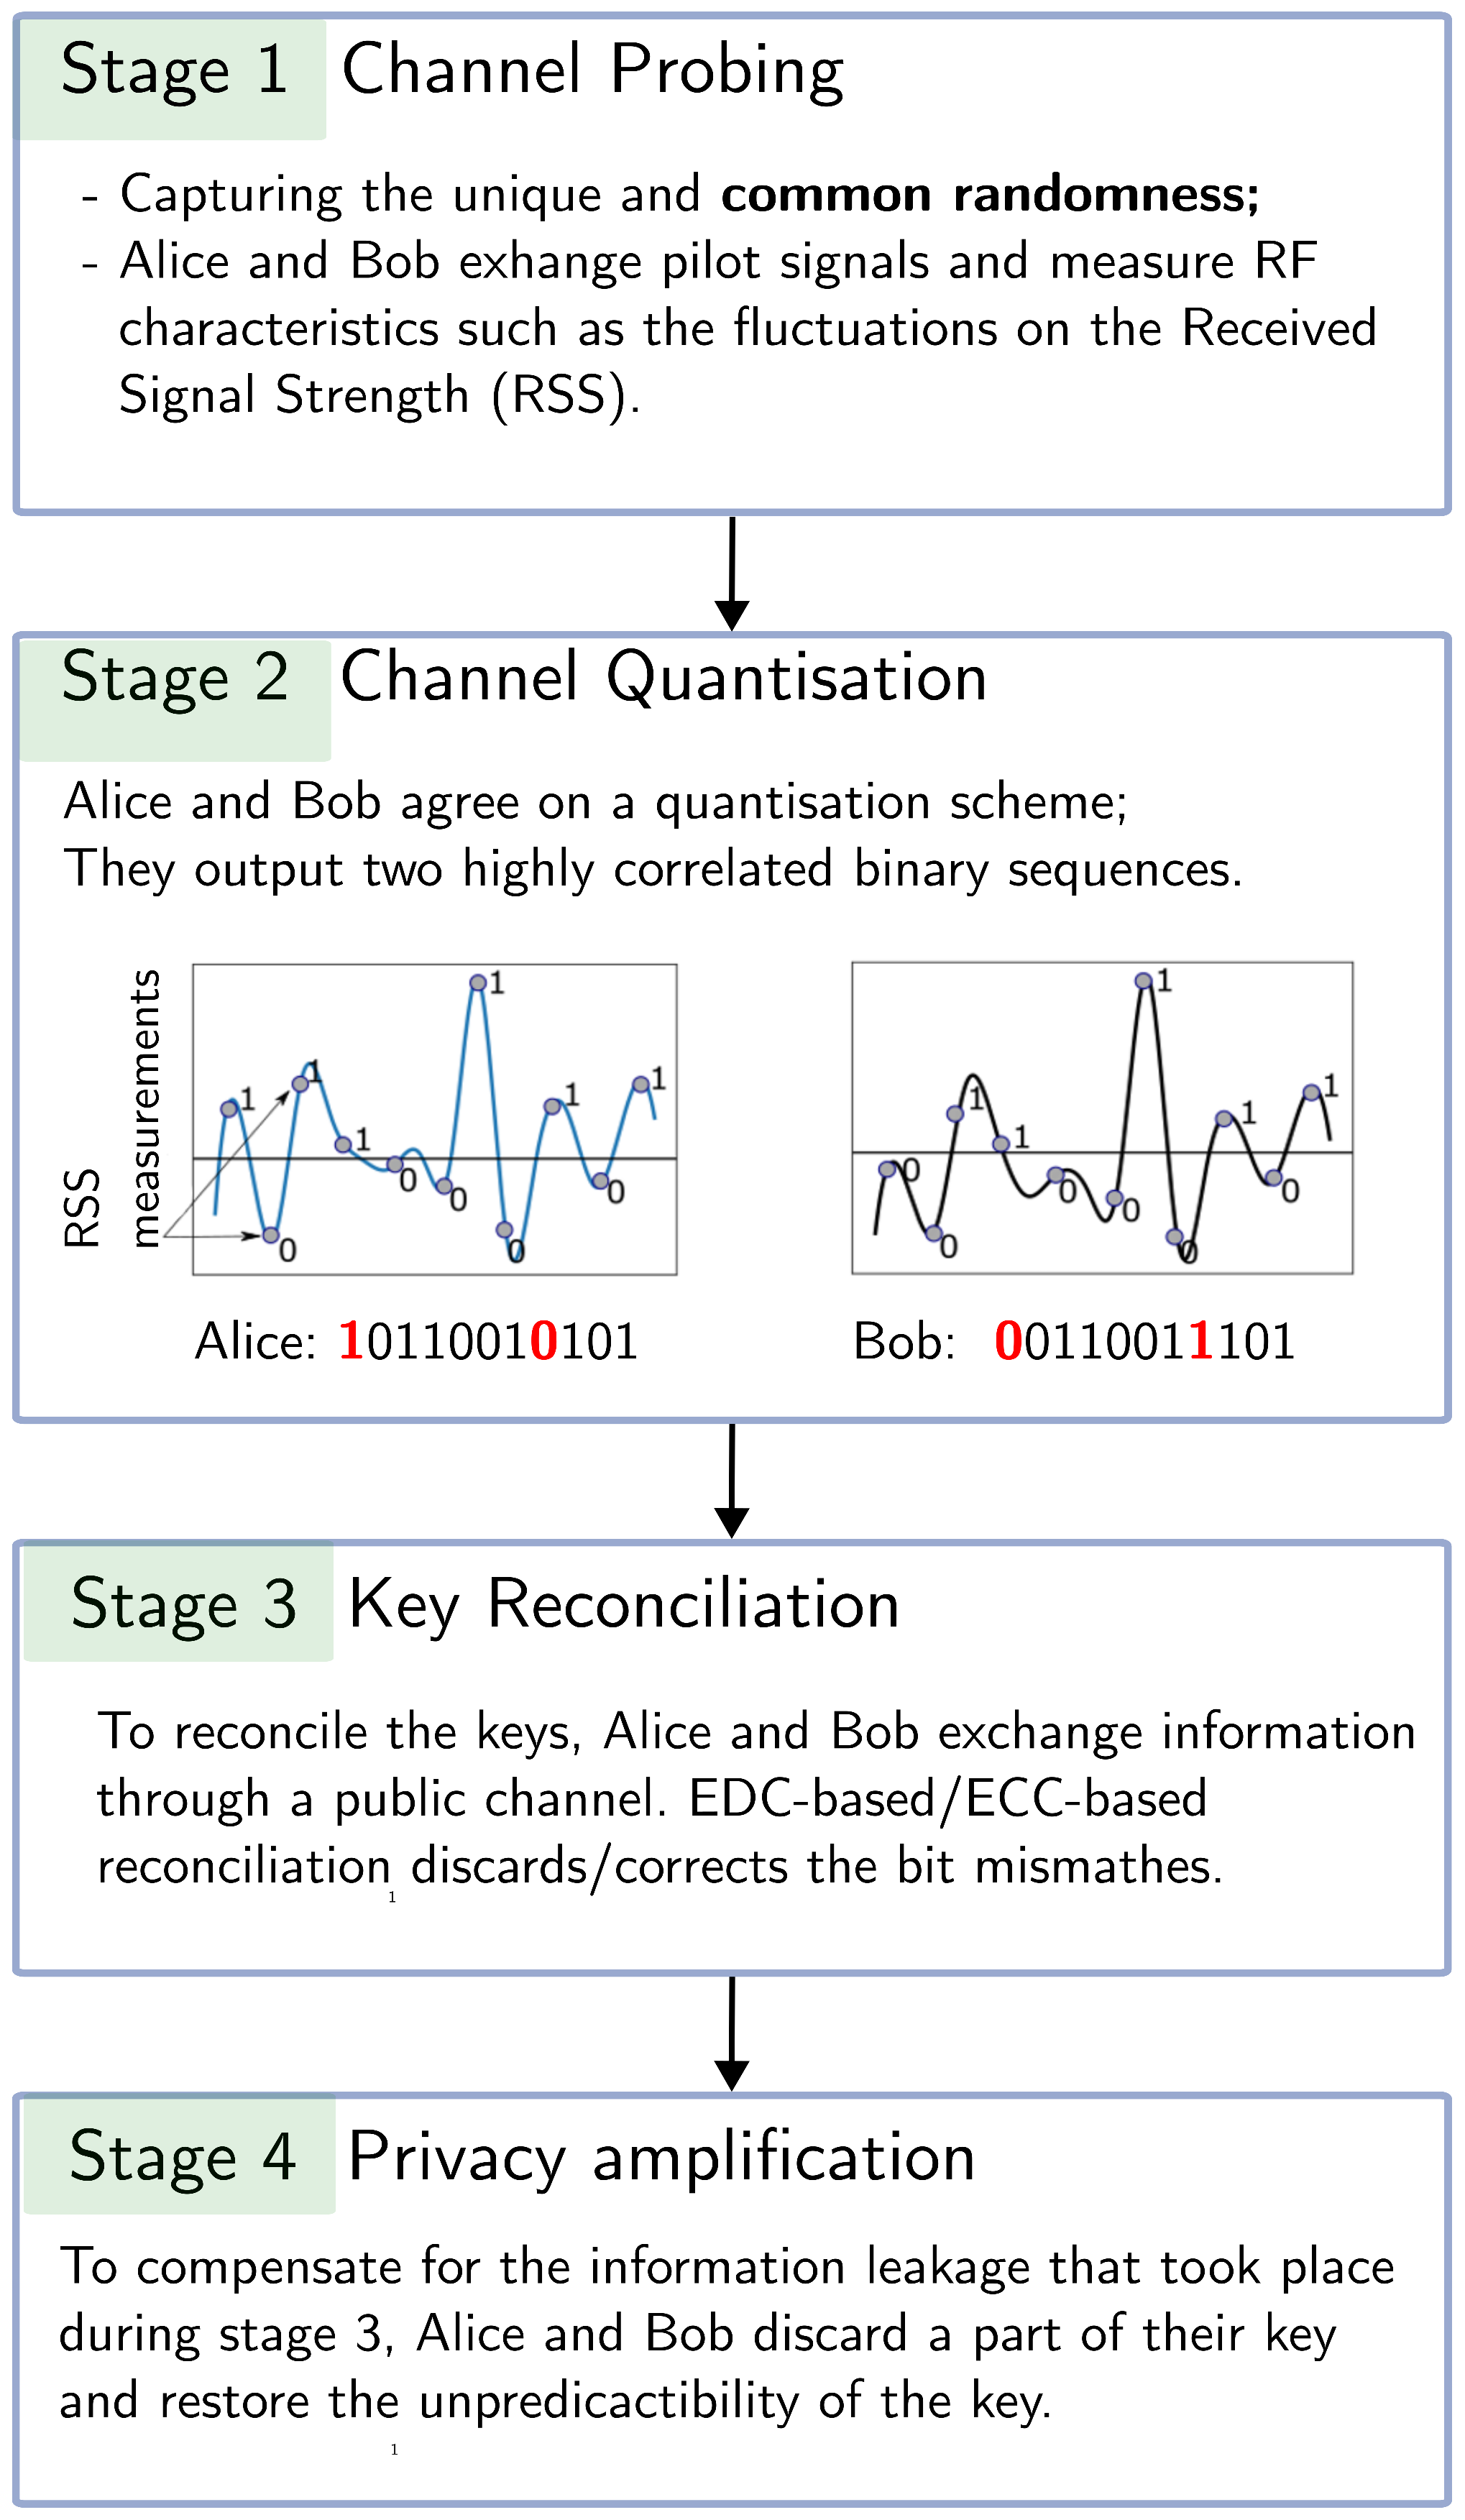
\includegraphics[scale = 0.215]{slides/figures/PLKG.eps}
    \caption{Caption}
    \label{fig:PLKG}
\end{figure}
\end{frame}

\begin{frame}{The four stages of physical layer key generation (cont.)}
    
\begin{figure}
    \centering
    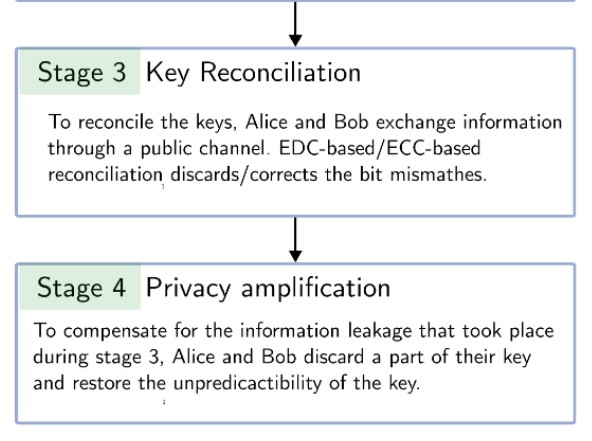
\includegraphics[scale = 0.7]{slides/figures/KGR2.jpg}
    \caption{The four stages of a typical physical layer key generation protocol.}
    \label{fig:PLKG2}
\end{figure}
\end{frame}


\begin{frame}{Limitations of PLKG}
    \begin{itemize}
        \item Low key rates when the wireless channel is not highly dynamic;
        \item Idealistic assumptions:
        \item Key reconciliation may be costly for small devices with little computational capabilities;
        
    \end{itemize}
\end{frame}


\subsection{Survey on physical layer authentication for short-range systems}

\begin{frame}{Authentication}
\begin{figure}
    \hspace*{-2.2cm}
    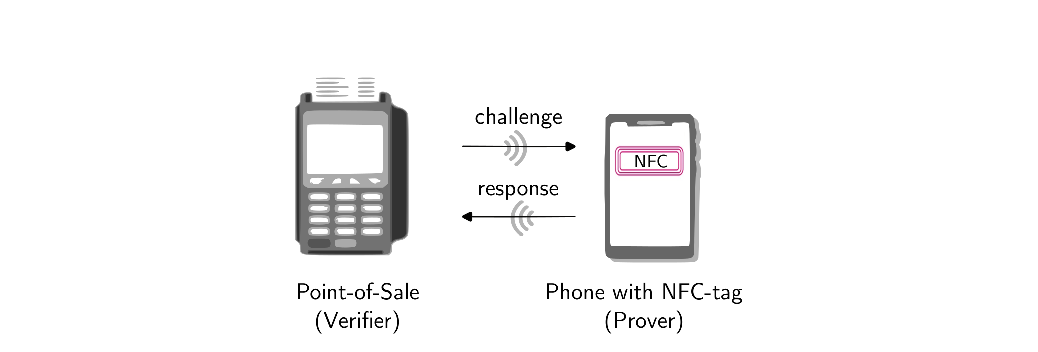
\includegraphics[scale=0.9]{slides/figures/NFC.eps}
    \caption{Verifier-prover example in NFC}
    \label{fig:NFC}
\end{figure}
    
\end{frame}

\begin{frame}{Relay/Replay attacks}
    \begin{figure}
    \hspace*{-1.3cm}
    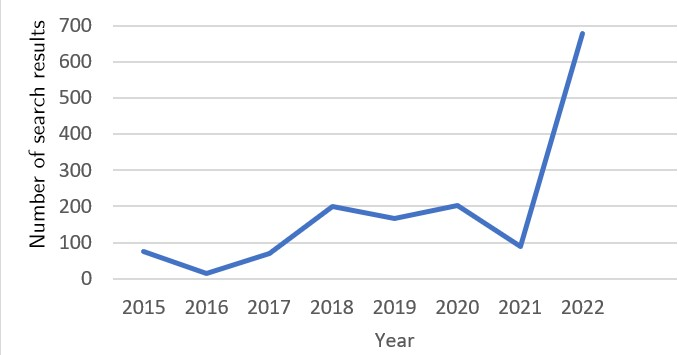
\includegraphics[scale = 0.85]{slides/figures/googleNews.jpg}
    \caption{Number of search results on Google News over the years. Search string: “replay
attacks” OR “relay attacks”}
    \label{fig:google_news}
\end{figure}
\end{frame}

\begin{frame}{Mafia-Fraud}
    \begin{figure}
    \hspace*{-2cm}
        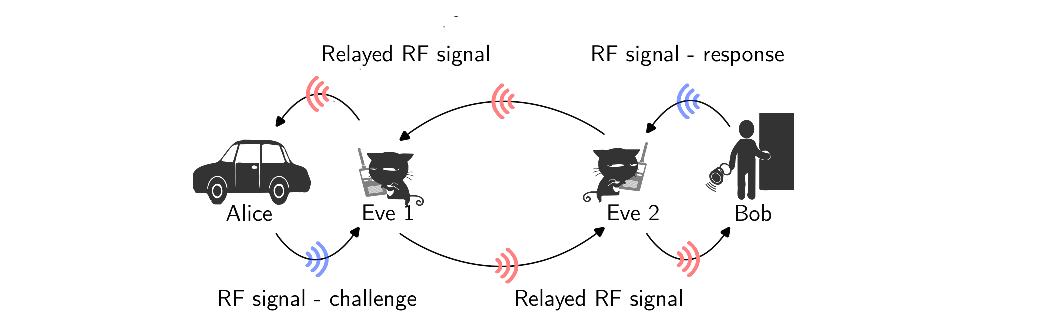
\includegraphics[scale = 0.9]{slides/figures/mafia_fraud.eps}
        \caption{A Mafia Fraud attack with two adversary nodes.}
        \label{fig:enter-label}
    \end{figure}
\end{frame}

\begin{frame}{Terrorist Fraud}
    \begin{figure}
        \centering
        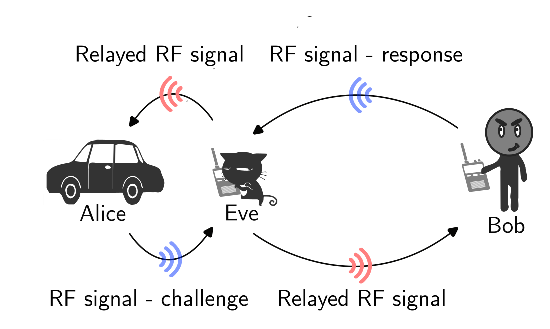
\includegraphics[scale = 0.9]{slides/figures/terrorist_fraud.eps}
        \caption{In a Terrorist Fraud attack, remote Bob cooperates with a local adversary node.}
        \label{fig:enter-label}
    \end{figure}
\end{frame}

\begin{frame}{Current Solutions and Limitations}
    \begin{itemize}
        \item Physical Layer Identification
        \item Time-of-flight distance bounding
        \item Ambient Conditions
        \item RSS and phase-based ranging
    \end{itemize}
    
\end{frame}



%%%%%%%%%%%%%%%%    OLD %%%%%%%%%%%%%%
\iffalse
\begin{frame}
\frametitle{}
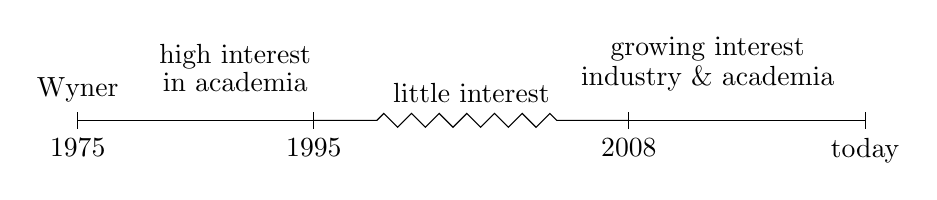
\begin{tikzpicture}[snake=zigzag, line before snake = 8mm, line after snake = 8mm]
    % draw horizontal line   
    \draw (0,0) -- (3,0);
    \draw[snake] (3,0) -- (7,0);
    %\draw (4,0) -- (5,0);
    \draw (7,0) -- (10,0);

    % draw vertical lines 1975,1995,2008,today
    \foreach \x in {0,3,7,10}
      \draw (\x cm,3pt) -- (\x cm,-3pt);

    % draw nodes
    \draw (0,0) node[below=3pt] {$ 1975 $} node[above=3pt] {Wyner};
    \draw (1,0) node[below=3pt] {$  $} node[above=3pt] {$ $};
    \draw (2,0) node[below=3pt] {$  $} node[above=15pt] {high interest}
    node[above=7pt] {in academia};
    \draw (3,0) node[below=3pt] {$  1995 $} node[above=3pt] {$  $};
    \draw (4,0) node[below=3pt] {$  $} node[above=3pt] {};
    \draw (5,0) node[below=3pt] {$  $} node[above=3pt] {little interest};
    \draw (6,0) node[below=3pt] {$ $} node[above=3pt] {$  $};
    \draw (7,0) node[below=3pt] {2008} node[above=15pt] {};
     \draw (8,0) node[below=3pt] {$ $} node[above=18pt] {growing interest}
     node[above=7pt]{industry \& academia};
    %\draw (9,0) node[below=3pt] {today} node[above=3pt] {};
    \draw (10,0) node[below=3pt] {today} node[above=3pt] {};
  \end{tikzpicture}
\end{frame}

\fi

\section*{}
\begin{frame}{}
\begin{beamercolorbox}[colsep=1.5pt,rounded=true,shadow=true]{block body example}
    \huge{Chapter 4: Key Generation and Spatial Separation}
\end{beamercolorbox}
\vspace{2cm}
\textbf{Publication}:\\
C. Paschou, O. Johnson, Z. Zhu, and A. Doufexi.``Re-Defining Secure Distance for CSI-based Key Generation Protocols.'' In 2022 IEEE 95th Vehicular Technology Conference (VTC2022-Spring), pp. 1-6. IEEE, 2022.




\end{frame}


\section{Key Generation and Spatial Separation}
\begin{frame}{Motivation}
\begin{itemize}
\item \textbf{Common assumption in key generation:} In a rich scattering environment, when Eve is positioned half a wavelength $(0.5\lambda)$ apart, her channel is decorrelated to Bob's.
    \item This chapter points out that a distance of $0.5\lambda$ is not perfectly secure, even in idealistic environments with rich scattering.
    \item \textbf{Novel contribution:} If the distance of $0.5\lambda$ is not perfectly secure, then what is?
    \item Three geometric environments are studied:
    \begin{itemize}
        \item Isotropic scattering
        \item Omnidirectional scattering
        \item Restricted Uniform Angle-of-Arrival
    \end{itemize}
\end{itemize}
\end{frame}

\begin{frame}{Channel Correlation and Secrecy Degradation}
\framesubtitle{Worst case scenario}
\begin{figure}
    \centering
    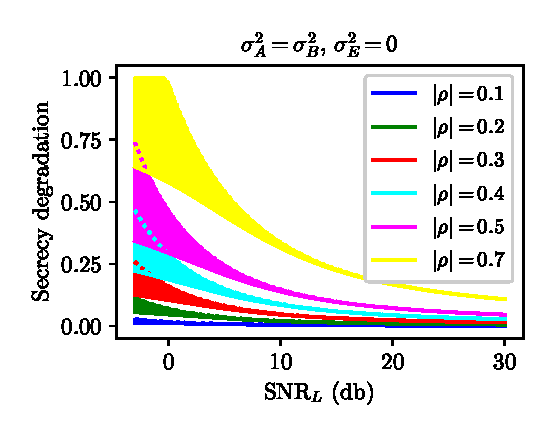
\includegraphics[scale = 0.9]{figures/key_generation_and_spatial_seperation/bounds_degrad.eps}
    \vspace{-0.5cm}
    \caption{Secrecy degradation as a function of $\rho$ and {SNR} at the legitimate users ($SNR_L = SNR_A = SNR_B$)}
\end{figure}
\end{frame}

\begin{frame}{Channel Correlation and Secrecy Degradation}
\framesubtitle{Equal SNR at all receivers}
\begin{figure}
    \centering
    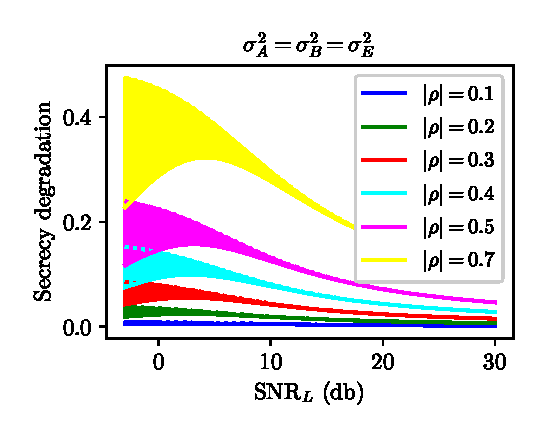
\includegraphics[scale = 0.9]{figures/key_generation_and_spatial_seperation/boundsDegrallequal.eps}
    \vspace{-0.5cm}
    \caption{Secrecy degradation as a function of $|\rho|$ and {SNR} at the legitimate users ($SNR_L = SNR_A = SNR_B$)}
\end{figure}
\end{frame}

\begin{frame}{Secure Distance}
\framesubtitle{Definition}    

\begin{definition}
    In a Cartesian coordinate system, let Eve be positioned at $E(x,y,z)$ and let $\rho(E(x,y,z))$ be the spatial channel correlation between Eve's channel and Bob's channel when Eve is positioned at $E(x,y,z)$. A distance $d_{s}$ is said to be $\epsilon$-secure if
    ~
    \begin{equation}
        |\rho(E(x,y,z))| < \epsilon \text{ for all } E(x,y,z)\notin S(B,d_s),
    \label{secure distance}\end{equation}
    where $S(B,d_{s})$ is the sphere with centre Bob's location and radius $d_{s}$. \label{dfn: secure distance}
\end{definition}
\end{frame}


\begin{frame}{Secure Distance}
\framesubtitle{Idealistic Scattering Environments}
\begin{figure}
    \centering
   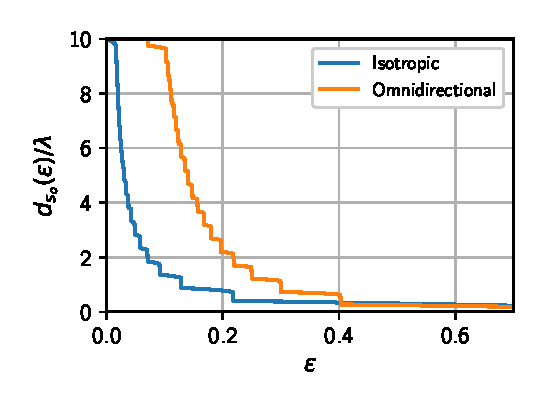
\includegraphics{figures/key_generation_and_spatial_seperation/securedistrichscattering.eps}
    \caption{The minimum secure distance for different thresholds.}
\end{figure} 
\end{frame}


%\begin{frame}{Secure Distance}
%\framesubtitle{Insights on the Derivation of Secure Distance}
%\begin{figure}
 %   \centering
  %  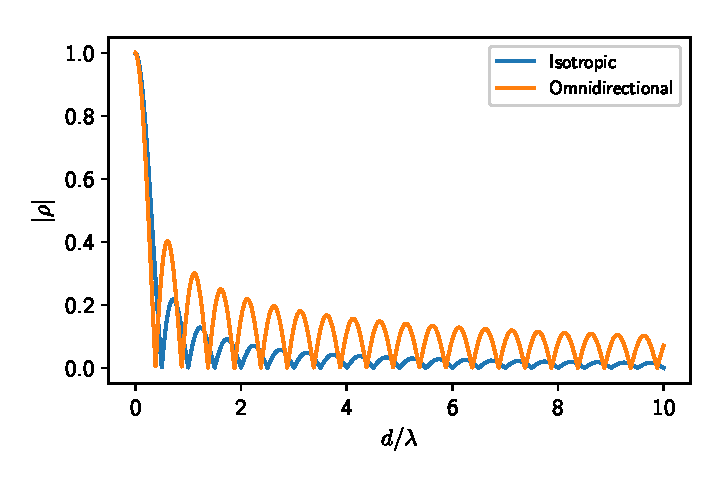
\includegraphics[scale = 0.78]{figures/key_generation_and_spatial_seperation/correlationRichscattering.eps}
   % \vspace{-0.5cm}
    %\caption{ The spatial channel correlation against the normalised distance between two
%receivers for the cases of isotropic diffuse field and omnidirectional diffuse field.}
%\end{figure}
%\end{frame}

\begin{frame}{Secure Distance}
\begin{example}
\textbf{Isotropic case:} The 0.1-secure distance is approximately 1.5$\lambda$.
\end{example}
\begin{example}
    \textbf{Omnidirectional case:} The 0.1-secure distance is approximately 10$\lambda$.
I.e., when Bob and Eve are equipped with dipole antennas, it takes approximately 10$\lambda$ for the channel correlation to drop below $0.1$.
\end{example}    
\end{frame}


\begin{frame}{Secure Distance}
\framesubtitle{Restricting the AoA}
\begin{figure}
    \centering
    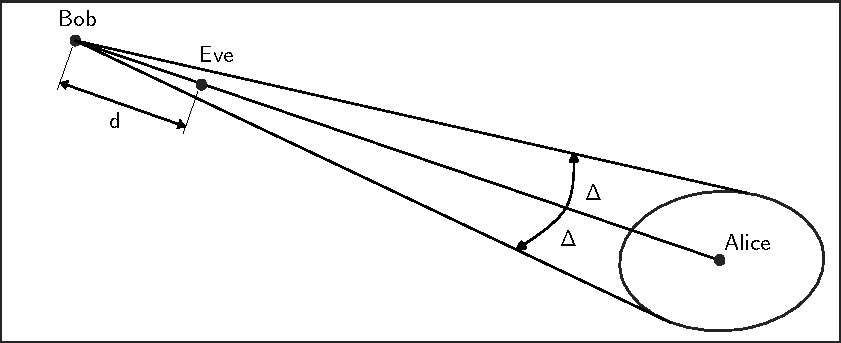
\includegraphics[scale = 0.7]{figures/key_generation_and_spatial_seperation/directional_optimal_eve.pdf}
    \caption{The restricted uniform AoA model. The spatial channel correlation maximises when Eve is inline with AB.}
    %\label{fig:enter-label}
\end{figure}    
\end{frame}

\begin{frame}{Secure Distance}
\framesubtitle{Restricting the Angle-of-Arrival}
\begin{figure}
    \centering
    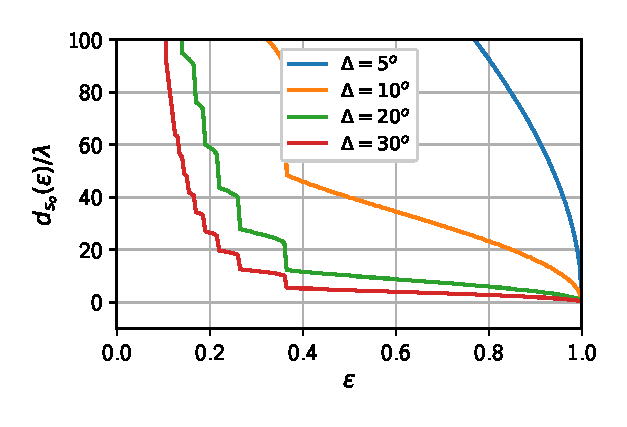
\includegraphics[scale = 0.9]{figures/key_generation_and_spatial_seperation/securedistDelta30zoom.eps}
    \caption{The minimum secure distance for different thresholds.}
   % \label{fig:enter-label}
\end{figure}
\end{frame}

\begin{frame}{Secure Distance}
\framesubtitle{Restricting the Angle-of-Arrival}
\begin{figure}
    \centering
    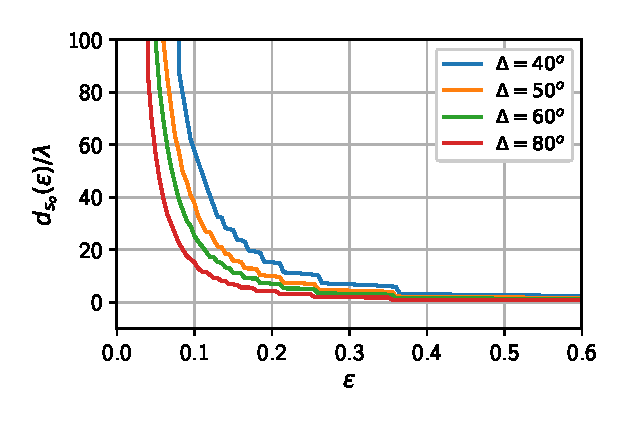
\includegraphics[scale = 0.9]{figures/key_generation_and_spatial_seperation/securedistDelta80zoom.eps}
    \caption{ Minimum secure distance such that the spatial correlation falls below $\epsilon$.}
\end{figure}
\end{frame}

\begin{frame}{Secure Distance}
\framesubtitle{Restring the Angle-of-Arrival}
\begin{figure}
    \centering
    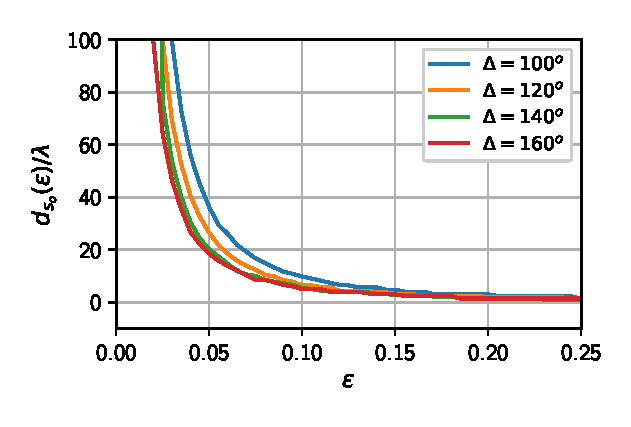
\includegraphics[scale = 0.9]{figures/key_generation_and_spatial_seperation/securedistDelta160zoom.eps}
    \caption{ Minimum secure distance such that the spatial correlation falls below $\epsilon$.}
    \label{fig:enter-label}
\end{figure}
\end{frame}

\begin{frame}{Secure Distance}
\framesubtitle{Restricting the Angle-of-Arrival}
 \begin{example}
Operating frequency: 2.4GHz
{AoA}-beamwidth: $80^0$ ($\Delta =40^o$). To achieve a maximal spatial correlation of 0.1, the eavesdropper needs to be distanced by at least 7m ($57\lambda$) from Bob. 
\end{example}

%\begin{example}
%Operating frequency: %$2.4GHz$
%{AoA}-beamwidth: $16^0$ ($\Delta =320^o$). To achieve a maximal spatial correlation of 0.1, the eavesdropper needs to be distanced by at least 2m ($19\lambda$) from Bob. 
%\end{example}
\begin{example}
For a minimum 0.1-secure distance of less than 1m, the beamwidth needs to be at least $200^o$ when the operating frequency is $f_c$=2.4GHz.
\end{example}
\end{frame}

\begin{frame}{Concluding Remarks}

\begin{itemize}
\item Even in an idealistic rich scattering, and assuming dipole antennas, the eavesdropper needs to be positioned at least ten wavelengths away to ensure negligible impact on secret key capacity;
\item In directive channels, the secure distance dramatically increases as the angle-of-arrival deviates from a uniform distribution across $(0, 2\pi]$;

\item \textbf{Suggestion:} For an effective and secure secrecy system, it is necessary to consider the influence of spatial channel correlation. Then restore the unpredictability of the key by eliminating the vulnerable key bits.

\end{itemize}   
\end{frame}

\section*{}
\begin{frame}{}
\begin{beamercolorbox}[colsep=1.5pt,rounded=true,shadow=true]{block body example}
    \huge{Chapter 5: Enabling a positive secrecy gap}
\end{beamercolorbox}
\vspace{2cm}
\textbf{Publications:}\\
 C. Paschou, O. Johnson, A. Doufexi, Z. Zhu, and W.H. Chin. ``Increasing the secrecy gap in quasi-static Rayleigh channels with secret splitting.'' In 2020 IEEE Globecom Workshops (GC Wkshps, pp. 1-7. IEEE, 2020.

\end{frame}

\section{Enabling a positive secrecy gap}


\begin{frame}{Motivation}
\title{How can we achieve confidentiality in non-static environments?}

\begin{itemize}
    \item Limitations of PL key-generation protocols: Slow-fading channels result in a low-key rate;

\item Vulnerability of PL key generation protocols: In directive channels, spatial channel correlation remains high over long distances. The eavesdropper may attain useful information about the key;

\item On the other hand \textbf{keyless PLS} does not rely on the spatial decorrelation property nor a dynamic channel but requires a \textbf{positive secrecy gap};

\end{itemize}
\end{frame}


\begin{frame}{Motivation}
\framesubtitle{The main limitation of keyless PLS}
    
\begin{figure}
\vspace{-1cm}
    \centering
    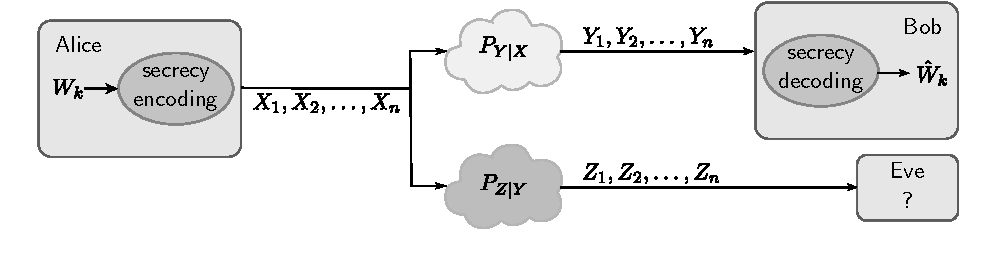
\includegraphics[scale = 0.65]{slides/figures/WiretapChannelCK.pdf}
    \vspace{-.5cm}
    \caption{The generic wiretap channel. Secure transmission is possible only when Bob experiences a better signal quality. I.e. a positive secrecy gap is needed.}
    \label{fig:CK}
\end{figure}
\vspace{-.5cm}
\begin{definition}
    Secrecy gap is the quality difference between the legitimate channel and the wiretap channel. 
\end{definition}

\end{frame}

\begin{frame}{Our solution}
\begin{itemize}
\item Address the requirement of a positive secrecy gap and apply keyless PLS for securely transferring small data such as keys;
\item Our method: Secret splitting utilises user cooperation and significantly increases the probability of a positive secrecy gap.

\end{itemize}. 
\end{frame}

\begin{frame}{Our solution}
\framesubtitle{Related work and differentiation}
The concept of secret splitting has its origins in \textbf{network coding}, but the proposed scheme focuses on using links created solely in the \textbf{physical layer}, particularly in the context of \textbf{distributed massive-MIMO and BS cooperation}.
    
\end{frame}

\begin{frame}{Secret Splitting}
Secret splitting relies on BS cooperation on the downlink and transmit beamforming.
    \framesubtitle{BS cooperation}
    \begin{figure}
        \centering
        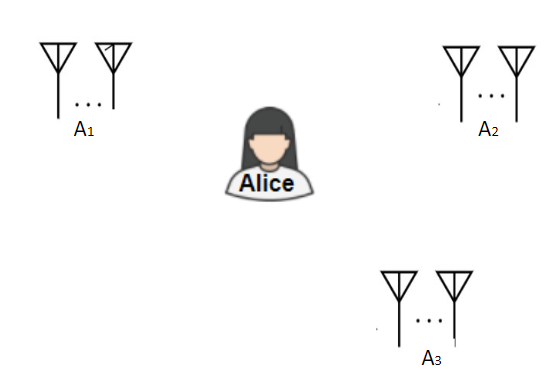
\includegraphics[scale=0.4]{figures/enabling_positive_secrecy_gap/SS_BS_cooperation.png}
        \caption{Alice is able to control two or more base stations.}
    \end{figure}
\end{frame}

\begin{frame}{Secret Splitting}
    \framesubtitle{Main Idea}

    The secret is split in multiple segments.\\
    Eve cannot be close to all transmitting nodes simultaneously. \\
    Eve is unable to reconstruct the secret.
    
    \begin{figure}
        \centering
        \includegraphics[scale=0.4]{figures/enabling_positive_secrecy_gap/SS_channel_model.PNG}
        \caption{Examplar case when Alice deploys two base stations. Bob reveals the secret by XORing the two splits.}
        \label{fig:enter-label}
    \end{figure}
\end{frame}

\begin{frame}{Secret Splitting}
    \framesubtitle{Probability of a positive secrecy gap.}

    \begin{figure}
        \centering
        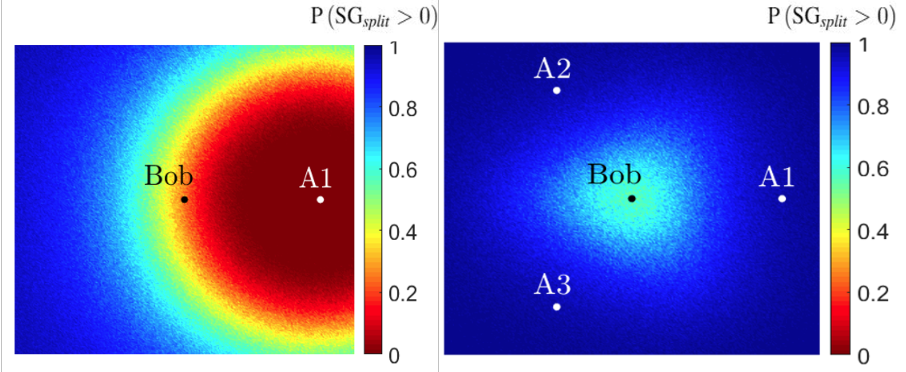
\includegraphics[scale=0.4]{figures/enabling_positive_secrecy_gap/SS_area.PNG}
        \caption{Left: conventional case without BS cooperation\\
        Right: Secret splitting with 3 BSs.}
        \label{fig:enter-label}
    \end{figure}
\end{frame}

\begin{frame}{Insights from Analysis}
\begin{itemize}

\item The secrecy capacity decreases linearly with the number of base stations;
\item Therefore, it is recommended to restrict secret splitting for the confidential transmission of keys;
\item When the total number of antennas is constrained, it is more beneficial to distribute the antennas at two BSs as long as the legitimate receiver is between them;
\item Therefore, the proposed scheme is a good fit for scenarios where the legitimate receiver moves along streets or railways.
\end{itemize}
\end{frame}

\begin{frame}{Concluding remarks}
\begin{itemize}
    \item Secret Splitting dramatically decreases the areas over which the eavesdropper has an advantage over the intended receiver;
    \item I.e., secret splitting enables a positive secrecy gap with a high probability;
    \item Secret splitting is recommended for the secure transmission of keys or other small data. 
\end{itemize}
    
\end{frame}

\section*{}
\begin{frame}{}
\begin{beamercolorbox}[colsep=1.5pt,rounded=true,shadow=true]{block body example}
    \huge{Chapter 6: Exploiting Channel Correlation against Distance Fraud}
\end{beamercolorbox}
\textbf{Publications:}\\
\begin{small}
    C. Paschou, O. Johnson, A. Doufexi, Z. Zhu, and W.H. Chin. ``Increasing the secrecy gap in quasi-static Rayleigh channels with secret splitting.'' In 2020 IEEE Globecom Workshops (GC Wkshps, pp. 1-7. IEEE, 2020.

    C. Paschou, O. Johnson, Z. Zhu, and A. Doufexi. ``A Lightweight Protocol for Validating Proximity in UHF RFID Systems.'' In 2021 IEEE 94th Vehicular Technology Conference (VTC2021-Fall), pp. 1-7. IEEE, 2021.

    C.Paschou, Z. Zhu, M. Sandell.
    ``Preventing replay/relay attacks in keyless entry systems.'' Patent 54322US, Oblon, McClelland, Maier \& Neustadt, {L.L.P.}, 2022.
    
    \end{small}

\end{frame}


\section{Exploiting channel correlation against distance fraud}

\begin{frame}{Motivation}
\framesubtitle{Authentication in short-range systems}

\begin{figure}
    \vspace{-1cm}
    \hspace*{-1.2cm}
    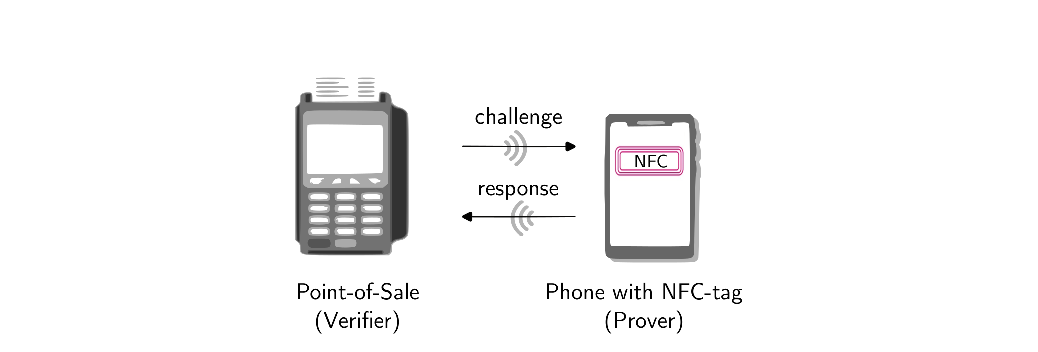
\includegraphics[scale=0.8]{slides/figures/NFC.eps}
    \caption{Verifier-prover example in NFC.}
    \label{fig:NFC}
\end{figure}
\vspace{-1cm}
\begin{beamercolorbox}[colsep=1.5pt,rounded=true,shadow=true]{block body alerted}{Current \textbf{short-range systems} are vulnerable to \textbf{distance fraud}.}
\end{beamercolorbox}
    
\end{frame}

\begin{frame}{Motivation}
\framesubtitle{Mafia-Fraud}
    \begin{figure}
    \hspace*{-2cm}
        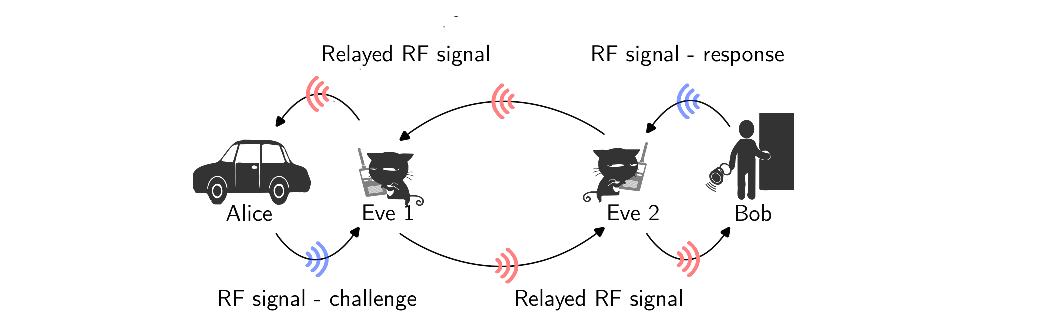
\includegraphics[scale = 0.9]{slides/figures/mafia_fraud.eps}
        \caption{A Mafia Fraud attack with two adversary nodes.}
        \label{fig:enter-label}
    \end{figure}
\end{frame}

\begin{frame}{Terrorist Fraud}
    \begin{figure}
        \centering
        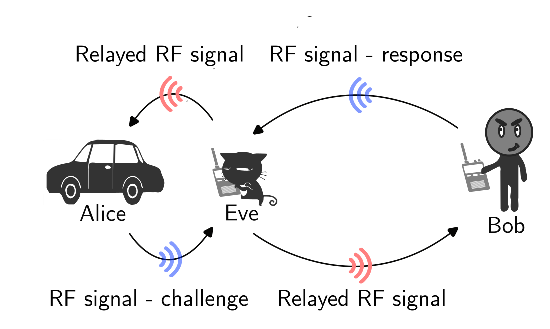
\includegraphics[scale = 0.9]{slides/figures/terrorist_fraud.eps}
        \caption{In a Terrorist Fraud attack, remote Bob cooperates with a local adversary node.}
        \label{fig:enter-label}
    \end{figure}
\end{frame}



\begin{frame}{Motivation}

\framesubtitle{Current Solutions and Limitations}
    \begin{itemize}
        \item Physical Layer Identification - promising solution against most distance fraud;
        \item Time-of-flight distance bounding - best solution but requires specialised hardware;
        \item Ambient Conditions - at least 5 sensor devices are needed;
        \item RSS and phase-based ranging - easy to implement but extremely vulnerable. AVOID.
    \end{itemize}
\vspace{2pt}
\begin{beamercolorbox}[colsep=1.5pt,rounded=true,shadow=true]{block body alerted}
A reliable method for narrowband and low-cost devices is missing.
\end{beamercolorbox}
\end{frame}

\begin{frame}{Motivation}
\framesubtitle{Our solution}

\begin{itemize}
\item Exploit the inherited properties of the RF channel: spatial/temporal correlation.
\item Two variants:
\begin{itemize}
    \item CHannel Randomness Yields Secure Proximity (\textbf{CHRYSP})
    \item against Solo-Distance RFID (\textbf{SD-RFID})
    \end{itemize}

\end{itemize}

    
\end{frame}


\begin{frame}{Motivation}
\framesubtitle{Our Solution vs Current Solution}
\begin{table}[ht!]
    \centering
    \begin{tabular}{|c|c|c|c|c|}
    \hline
     & Replay& Solo Dist.& Mafia& Terrorist\\
      & attack& Fraud& Fraud& Fraud\\
     %\hline
     %Crypt. methods & \checkmark& X& X&X   \\
     \hline
     RF fingerprints & \checkmark& X& \checkmark& \checkmark\\
     \hline
     Ambient Conditions & \checkmark& \checkmark&\checkmark & X\\
        \hline
     Time-of-flight& X& \checkmark &\checkmark & {\small{depends on}}\\
     dist. bound.&&&&\small{protocol}\\
     \hline
     CHRYSP & \checkmark & \checkmark &\checkmark & X\\
     \hline
     SDF-RFID & \checkmark & \checkmark &X& X\\
     \hline
    \end{tabular}
        \caption{Possibility for protection against authentication attacks in short-range communication systems}
    \label{tab:attacks}
\end{table}

\end{frame}


\begin{frame}{CHRYSP}
\framesubtitle{Channel Model}
\begin{figure}
    \centering    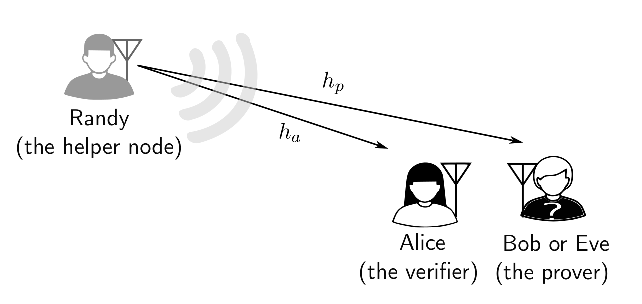
\includegraphics{figures/against_distance_fraud/RandyAliceChannelmodel.eps}
    
    \caption{Randy, Alice and Bob/Eve play the role of the helper node, the verifier, and the prover, respectively.}
\end{figure}
\end{frame}
%%%%%
\begin{frame}
\centering
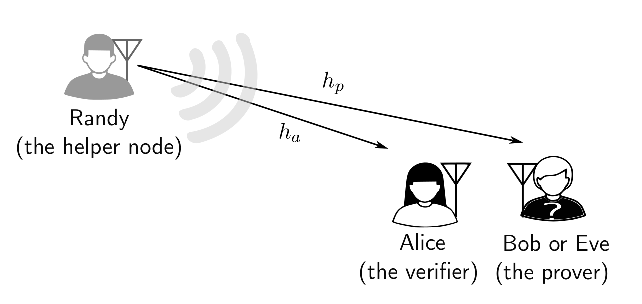
\includegraphics[width=0.6\linewidth]{figures/against_distance_fraud/RandyAliceChannelmodel.eps}

\begin{enumerate}
\item<1-> \textit{Channel measurements.}
Randy transmits known symbols. 
Alice \& prover record $N$ independent realisations of $h_a$ and $h_p$. Alice's and prover's channel sequences: $\{h_a[i]\}$, $\{h_p[i]\}$.

\item<2-> \textit{Signature.} The prover signs the channel sequence. Both channel sequence and signature are sent to Alice.


\item<3-> \textit{Legitimacy test.} Alice checks the validity of the signature.

\item<4-> \textit{Proximity test.} Alice estimates the channel correlation  $R(h_a, h_p)$. For a given threshold $\tau$:
\begin{align}
    &\text{If } |\hat{R}|\geq \tau, \text{ accept the prover}; \nonumber\\
    &\text{Otherwise}, \text{ reject the prover}.\nonumber
\end{align}
\end{enumerate}
\end{frame}

%%%%%%%%%%%%%%%%%%%%%%%%%%%%%%%%%%

\begin{frame}{SD-RFID}
\framesubtitle{Channel model}
\begin{figure}
    \vspace{-1cm}    
    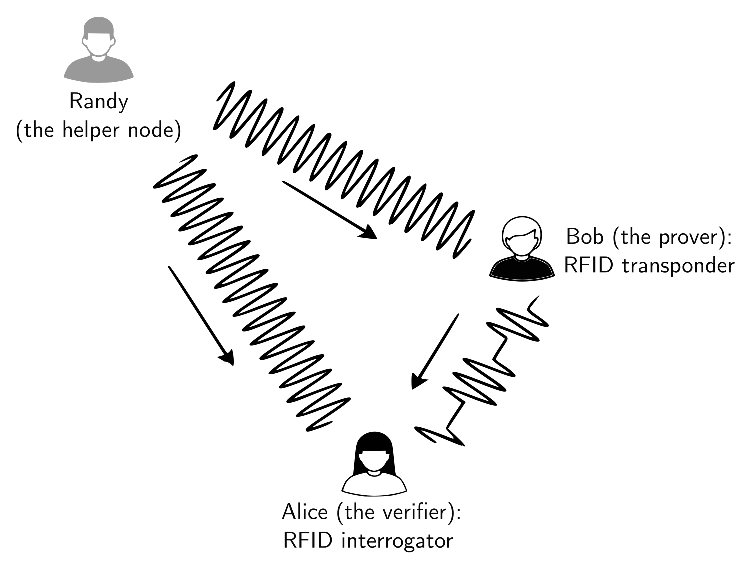
\includegraphics[scale = 0.6]{figures/against_distance_fraud/superposition.eps}
    \caption{The interrogator receives the superposition of two transmitting signals. At times when the transponder does not reflect the interrogator evaluates the channel $h_a$, whereas $h_b$ is measured during reflection.}
    \label{fig:enter-label}
\end{figure}
    
\end{frame}

\begin{frame}{Concluding Remarks}
\begin{itemize}
    \item The spatial channel correlation properties can be exploited to prove proximity.

    \item Under perfect channel estimation, the suggested method is a promising solution against relay attacks in non-static environments.

    \item A channel rich in entropy allows the required minimum channel correlation to be a small value, thereby enabling authentication over longer distances.

\end{itemize}
\end{frame}

\begin{frame}{Methodology}
\begin{enumerate}
    \item \textit{Data transmission.} Bob transmits typical data to Alice by using backscattering modulation on Randy's signal; 
    \item \textit{Channel measurements.} By applying signal processing techniques, Alice estimates both her own channel and Bob's channel. 
    \item \textit{Proximity Test.} Alice estimates the spatial channel correlation and approves or rejects the prover accordingly.  
\end{enumerate}
    
\end{frame}

\begin{frame}{Differences between SD-RFID \& CHRYSP}
\centering
\begin{tabular}{|p{2.5cm}|p{4cm}|p{3.5cm}|}
\hline
& \textbf{SD-RFID} & \textbf{CHRYSP} \\
\hline

\textbf{at the prover} & performs backscattering & RF antenna \\
 & seamless application & additional actions\\
\hline
\textbf{resilience} & SD-fraud & SD-fraud \\
 against& replay attack & replay attack \\
 \textbf{attacks}&               & Mafia Fraud \\
\hline

\end{tabular}
    
\end{frame}

\begin{frame}{Numerical Results}
\begin{figure}
    \centering
    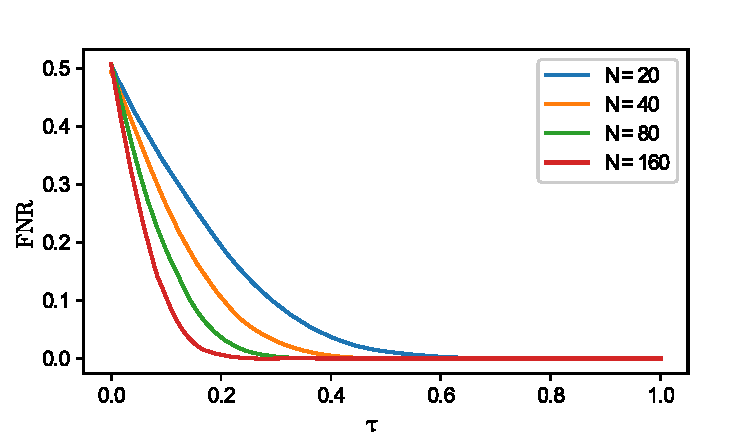
\includegraphics[scale = 0.8]{figures/against_distance_fraud/FNR_protect.eps}
    
    \caption{False-negative rate against the decision threshold}
\end{figure}
\end{frame}


\begin{frame}{Numerical Results}
\begin{figure}
    \centering
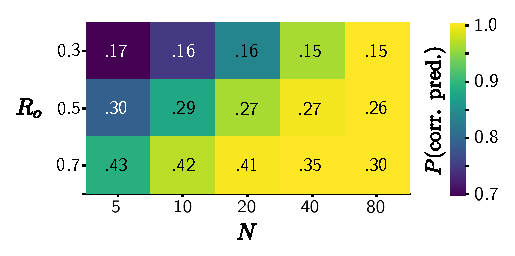
\includegraphics{figures/against_distance_fraud/colourmap_inkscape.eps}
\caption{Optimal thresholds for increasing the probability of correct predictions.}
\end{figure}
        
\end{frame}

\begin{frame}{Numerical Results - Insights}
\begin{itemize}

    \item Under perfect channel estimation and non-static environments, CHRYSP and SDF-RFID can protect against authentication attacks in short-range systems;
    \item A channel rich in entropy allows the required minimum channel correlation to be a small value, thereby enabling authentication over longer distances;
    

\end{itemize}

\end{frame}

\begin{frame}{Concluding Remarks}
\begin{itemize}

    \item Motivated by real-life authentication attacks in short-range systems, a novel concept has been introduced:\\
    Exploit channel correlation
    \item No specialised hardware, multiple sensors, or UWB systems are required except for the existence of a helper node and a non-static environment;
    \item Proposed methods are a good fit for resource-constrained short-range systems.
    

\end{itemize}

\end{frame}




\section*{}
\begin{frame}{}
\begin{beamercolorbox}[colsep=1.5pt,rounded=true,shadow=true]{block body example}
    \huge{Chapter 7: Channel Reciprocity for Key Transmission (CRicKET)}
\end{beamercolorbox}
\vspace{2cm}
\textbf{Publications}:\\
C. Paschou, F. Raimondo, M. Gugala, D. McEwan, J. Pope, G. Oikonomou.
    ``CRICKET: A Practical Physical Layer Key Agreement Protocol for IoT Networks.'' In 2023 IEEE International Conference of Communications (IEEE ICC 2023), pp. 1-7. IEEE, 2023.

\end{frame}

\section{Channel Reciprocity for Key Transmission (CRicKET)}

\begin{frame}{Motivation}
\framesubtitle{The four stages of physical layer key generation}
\vspace{-.26cm}
\begin{figure}
    \centering
    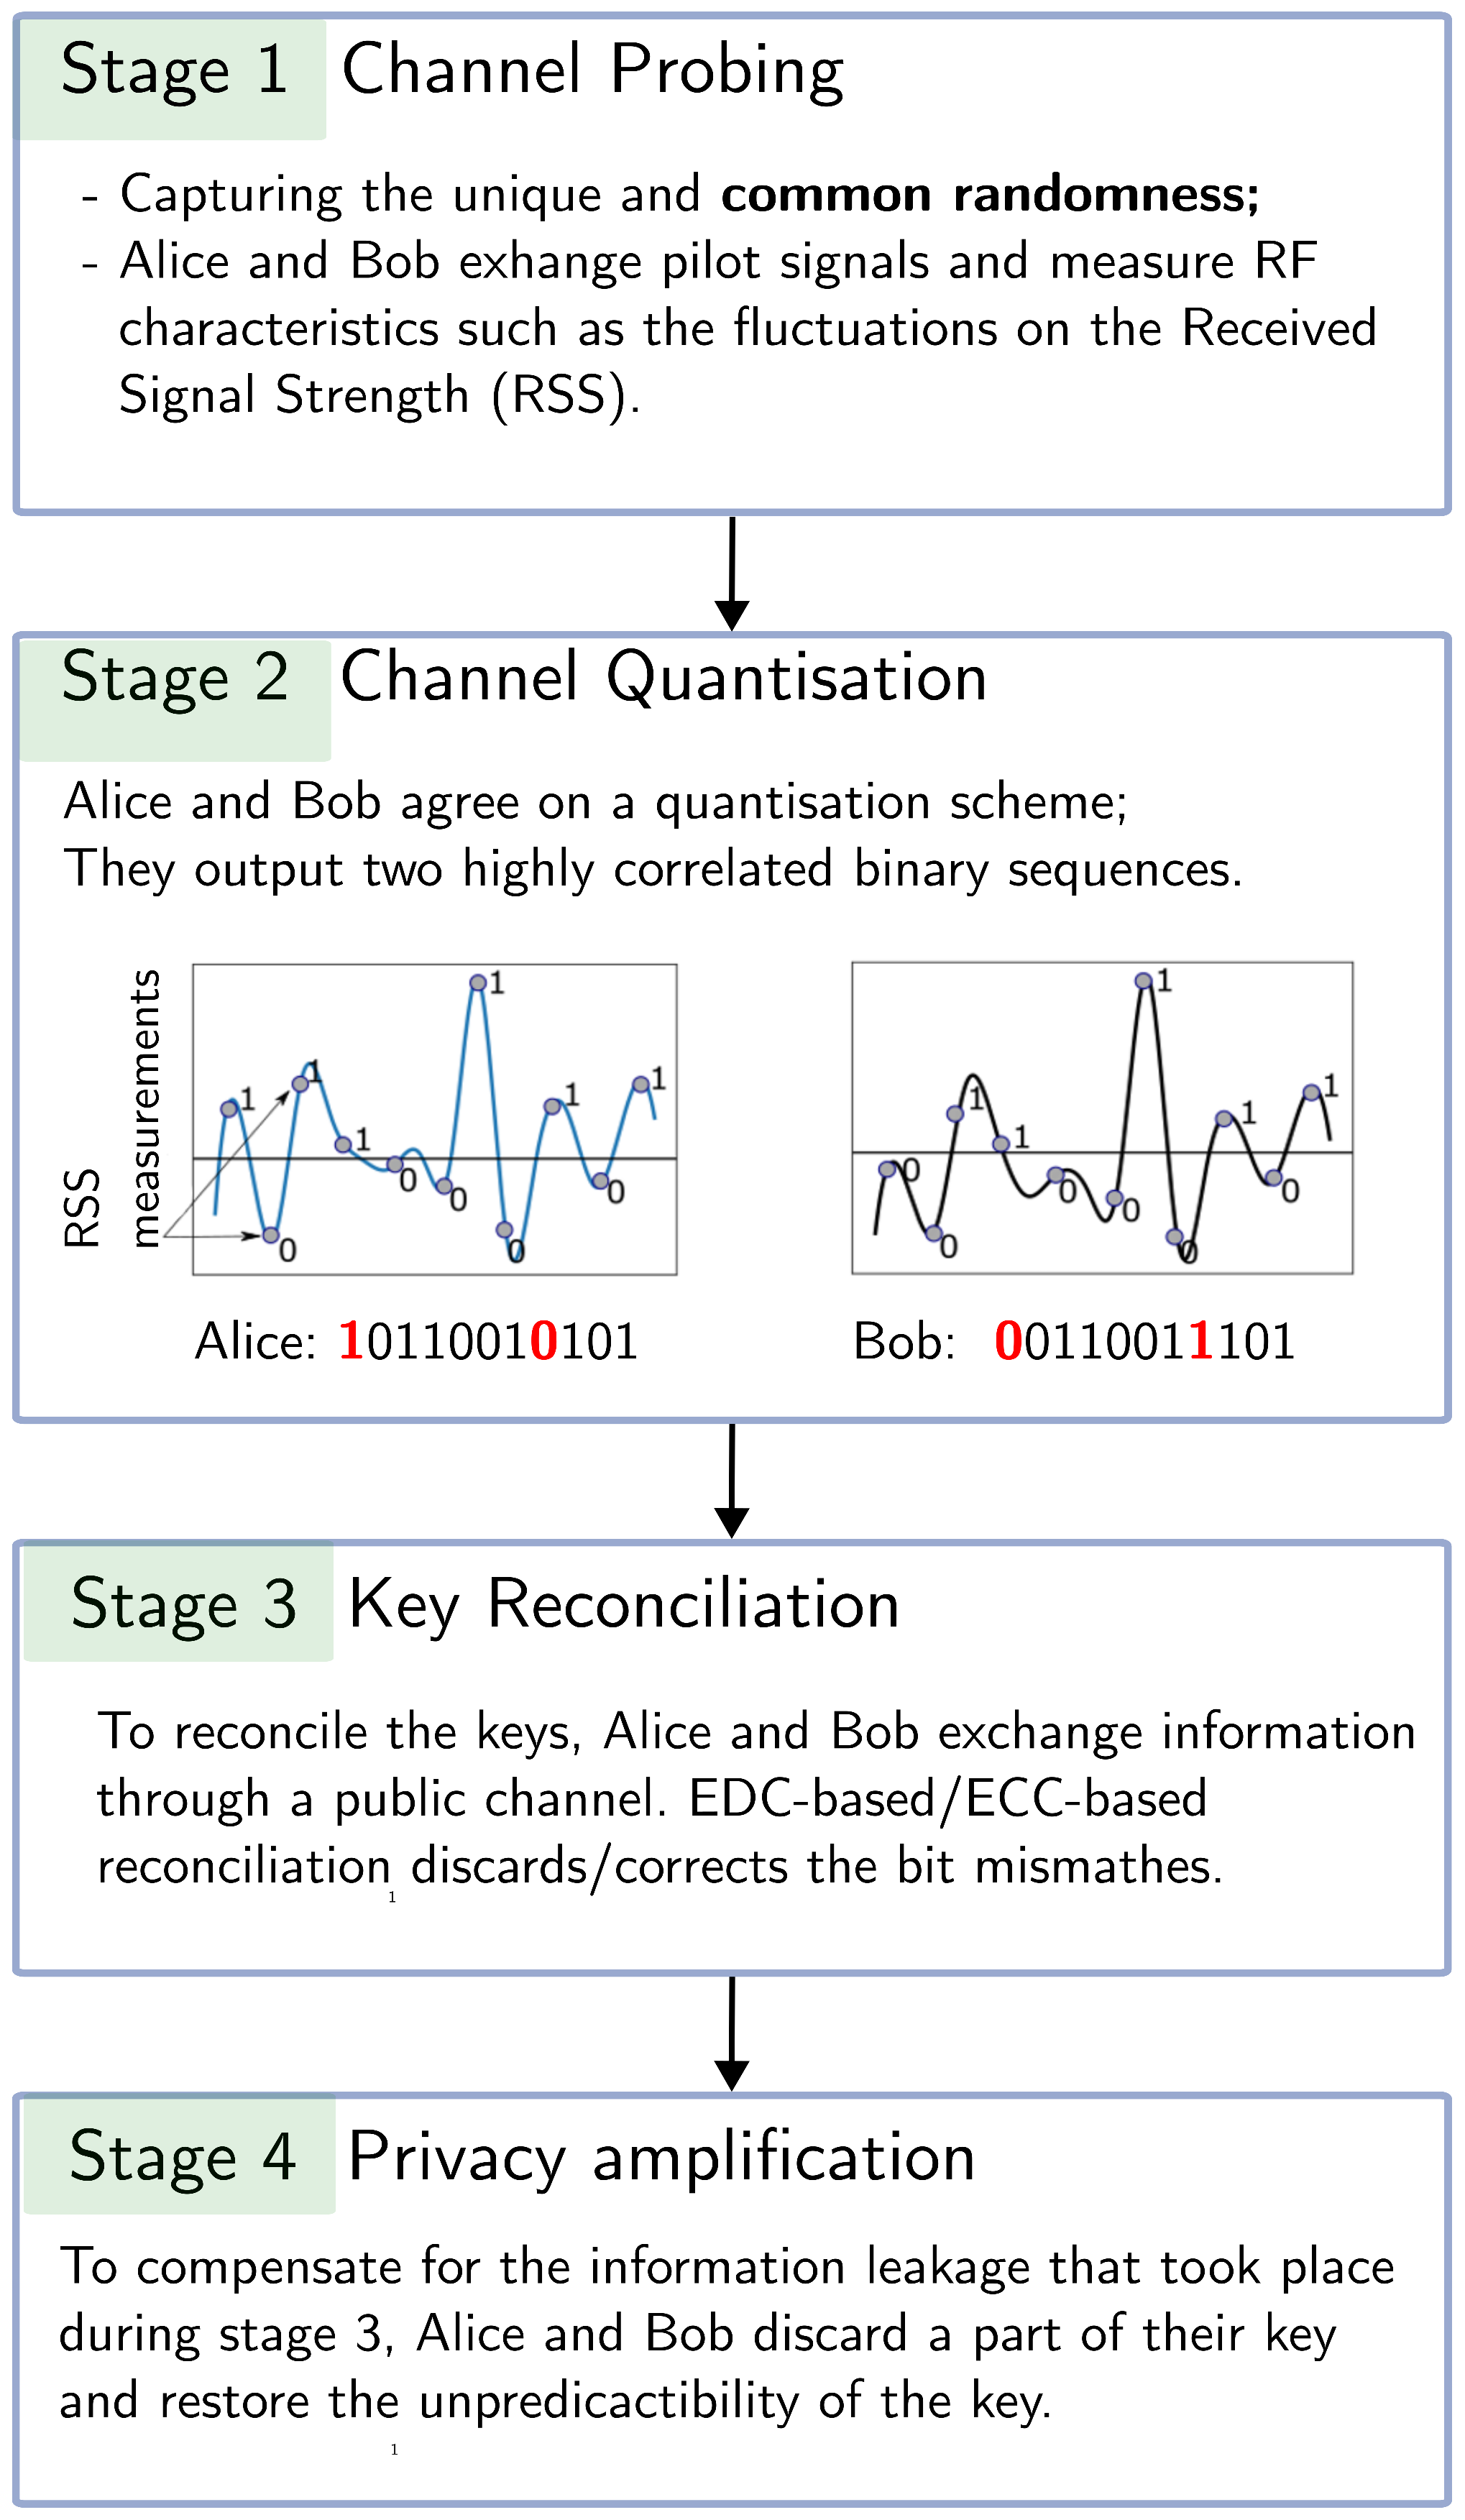
\includegraphics[scale = 0.215]{slides/figures/PLKG.eps}
    \caption{Caption}
    \label{fig:PLKG}
\end{figure}
\end{frame}

\begin{frame}{Motivation}
\framesubtitle{The four stages of physical layer key generation (cont.)}
\vspace{-.5cm}
\begin{figure}
    \centering
    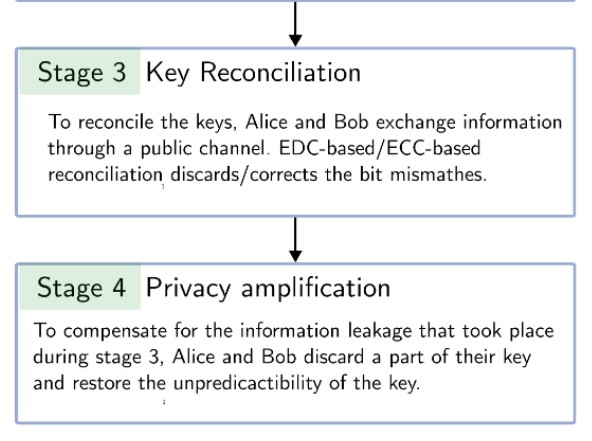
\includegraphics[scale = 0.7]{slides/figures/KGR2.jpg}
    \caption{The four stages of a typical physical layer key generation protocol.}
    \label{fig:PLKG2}
\end{figure}
\end{frame}


\begin{frame}{Motivation}
\framesubtitle{Current Limitations of Physical Layer Key Generation Protocols}
\begin{itemize}
    \item With typical Physical Layer Key Generation (PLKG):\\ high key disagreement rate $\rightarrow$ high reconciliation cost;
    \item High reconciliation cost $\rightarrow$ PLKG is impractical in resource-constrained networks.    
\end{itemize}
\begin{table}
    \centering
    \begin{tabular}{|c|ccc|}
    \hline
        \textbf{Approach} & \textbf{Comm.Overhead} & \textbf{Complexity} & \textbf{Leakage} \\
        \hline
        EDC-based & High & Low & Low\\
        ECC-based & Low & High & High\\
        \hline
    \end{tabular}
    \caption{A high-level comparison between EDC-based approaches and ECC-based approaches for key reconciliation.}
\end{table}
\end{frame}

\begin{frame}{Motivation}
\framesubtitle{Solution}
\begin{itemize} 
    \item CRicKET is a coding scheme for key transfer that keeps the key disagreement rate (KDR) arbitrarily low;
    \item Arbitrarily low KDR $\rightarrow$ arbitrarily low reconciliation cost;
    
    \item A low reconciliation cost trades off on encoding rate and not on computational complexity;
    \item CRicKET is a good fit for delay-tolerant applications with low computational capabilities. 
\end{itemize}
\end{frame}

\begin{frame}{CRicKET}
\begin{figure}
    \centering
    \vspace{-1.25cm}
    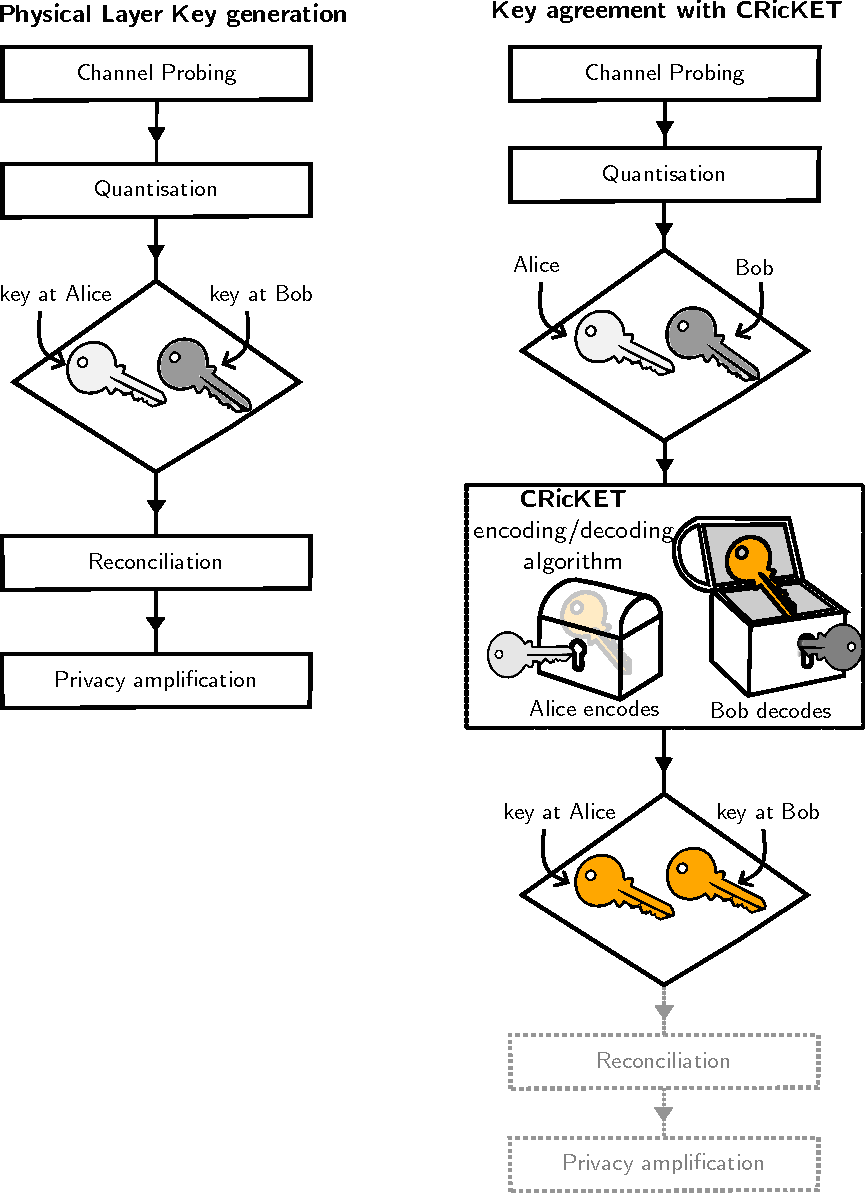
\includegraphics[scale = 0.4]{figures/Cricket/cricket vs PLKGv2.pdf}
    \caption{PLKG vs CRicKET}
    \label{fig:enter-label}
\end{figure}    
\end{frame}

\begin{frame}{Tunable parameters}
\begin{block}{Notation and Terminology}
\begin{beamercolorbox}[rounded=true]{block body}\textbf{Channel sequence}: the sequence obtained during the channel probing phase; \\
\textbf{Channel mismatch} ($p_{\text{ch}}$): measure of the difference between the channel sequence at Bob and the channel sequence at Alice;\\
$\mathbf{n}$, $\mathbf{\tau}$: coding parameters.
\end{beamercolorbox}
\end{block}

\begin{table}
    \centering
    \begin{tabular}{|c||ccccccccc|}
        \hline
       $p_{\text{ch}}$  & 0.05 & 0.1& 0.15&0.2 &0.25&0.3 &0.35&0.4 &0.45\\
        \hline
         \hline
       $n$ & 3& 5& 4 & 10& 15& 19& 28 &35& 54\\
        \hline
       $\tau$ & 0 & 0 & 0& 3 & 5& 6& 9& 9& 9 \\
        \hline
    \end{tabular}
    \caption{Optimal parameters for different values of $p_{\text{ch}}$ when the system's requirement is KDR < 0.001.}
    \label{tab: optimal}
\end{table}
\end{frame}

\begin{frame}{Encoding Rate vs Channel Miss-match}
\framesubtitle{}

\begin{figure}
    \centering
    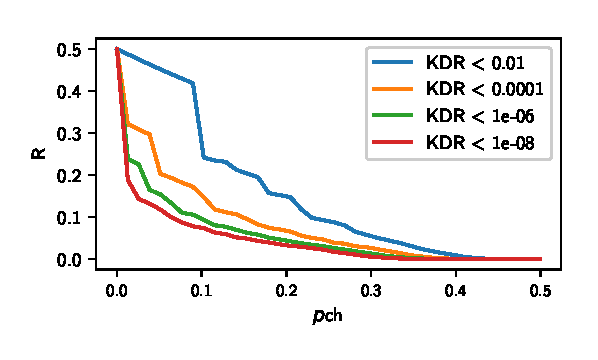
\includegraphics[scale = 0.9]{figures/Cricket/optimal_param.eps}
    \caption{Achievable encoding rates against channel mismatch for different requirements for the key disagreement rate.}
    \label{fig:acheivable rates}
    \end{figure}
\end{frame}

\begin{frame}{Implementation}
\begin{figure}
    \centering
    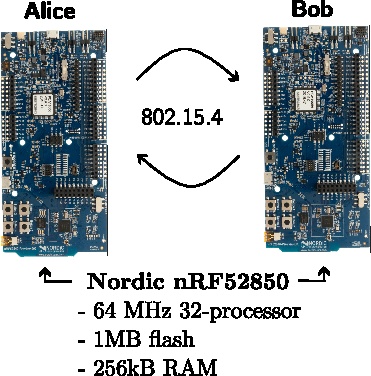
\includegraphics[scale = 0.9]{figures/Cricket/devices2.pdf}
    \caption{Caption}
    \label{fig:enter-label}
\end{figure}
    
\end{frame}

\begin{frame}{Implementation}
\begin{figure}
    \centering
    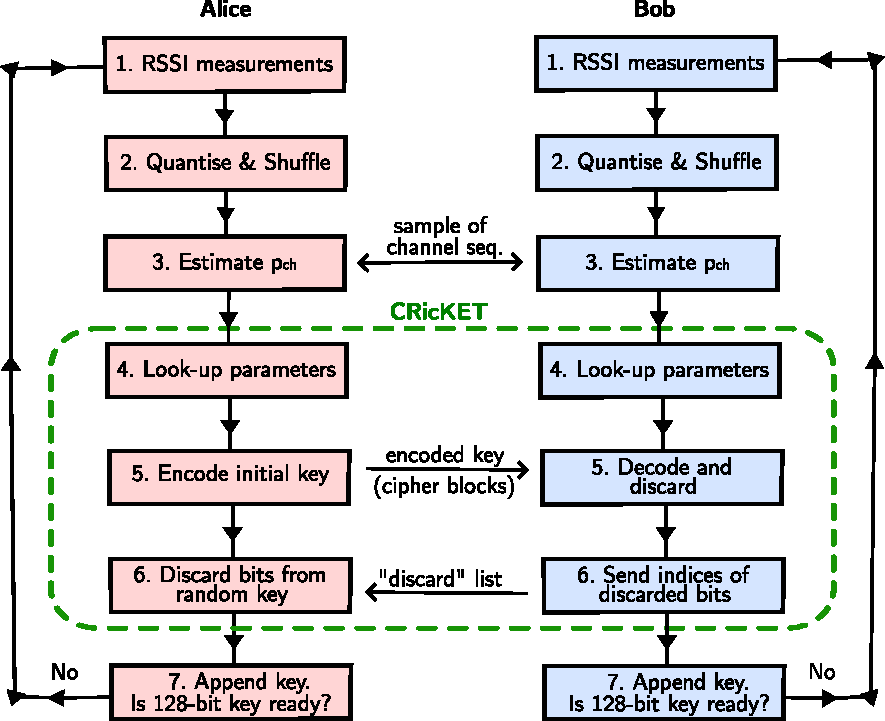
\includegraphics[scale = 0.5]{figures/Cricket/cricket_implentation.pdf}
    \caption{Flow diagram.}
    \label{fig:enter-label}
\end{figure}
\end{frame}

\begin{frame}{Implementation}
\framesubtitle{Experimental Results}
\begin{figure}
    \centering
    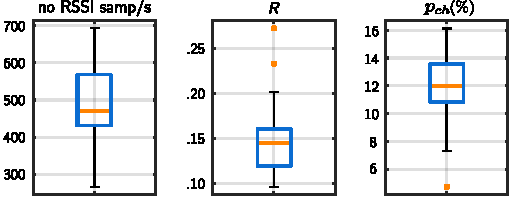
\includegraphics[scale = 1.2]{figures/Cricket/boxplots.pdf}
    \caption{Caption}
    \label{fig:enter-label}
\end{figure}
\end{frame}

\begin{frame}{Information Theoretic Guarantees}

\begin{itemize}
    \item CRicKET is proven to achieve perfect secrecy even when the channel sequences have low entropy \footnote{Under the assumption of decorrelated fading. I.e., Eve is assumed to be sufficiently distanced from the legitimate receivers.};
    \item By combining CRicKET with a high-level quantisation scheme or a ``smoothening'' filtering mechanism, it is possible to increase the key rate and decrease the vulnerability to brute-force attacks.
\end{itemize}
\end{frame}

\begin{frame}{Concluding Remarks}
\begin{itemize}
    \item {CRicKET} is a key agreement protocol designed for low-cost devices due to its minimal computational complexity and low memory requirements.

\item The parameters of {CRicKET} can be configured to achieve a desired key disagreement rate, and its analytical results have been validated.
\item A practical implementation over a low-rate wireless personal area network has demonstrated its suitability for IoT devices.
\end{itemize}
    
\end{frame}

\section*{}
\begin{frame}{}
\begin{beamercolorbox}[colsep=1.5pt,rounded=true,shadow=true]{block body example}
    \huge{Thesis Conclusion}
\end{beamercolorbox}
\end{frame}


\section{Thesis Conclusion}
\begin{frame}{}
\begin{itemize}

\item A cross-over approach is promoted, utilising the physical layer for key generation to facilitate upper-layer encryption;
\item Novel methods, such as secrecy splitting and CRicKET, address challenges in keyless and key-based PLS, respectively;
\item Exploiting spatial channel correlation is introduced for authenticating co-located devices, leading to methods CHRYSP and SDF-RFID.    
\end{itemize}
\end{frame}

\begin{frame}{Endnote}
  The state-of-the-art in PLS has been furthered, thus providing a viable basis for security enhancement to wireless networks of small devices.  
\end{frame}


\end{document}


